\par Ce chapitre contient les diagrammes de classes représentant le logiciel codé. Les diagrammes de l'itération trois ont été complétés à partir du code pour ajouter les détails d'intégration dans le diagrammes (méthodes privées par exemple).

\section{Paquetage interpreteurlir.donnees(.litteraux)}
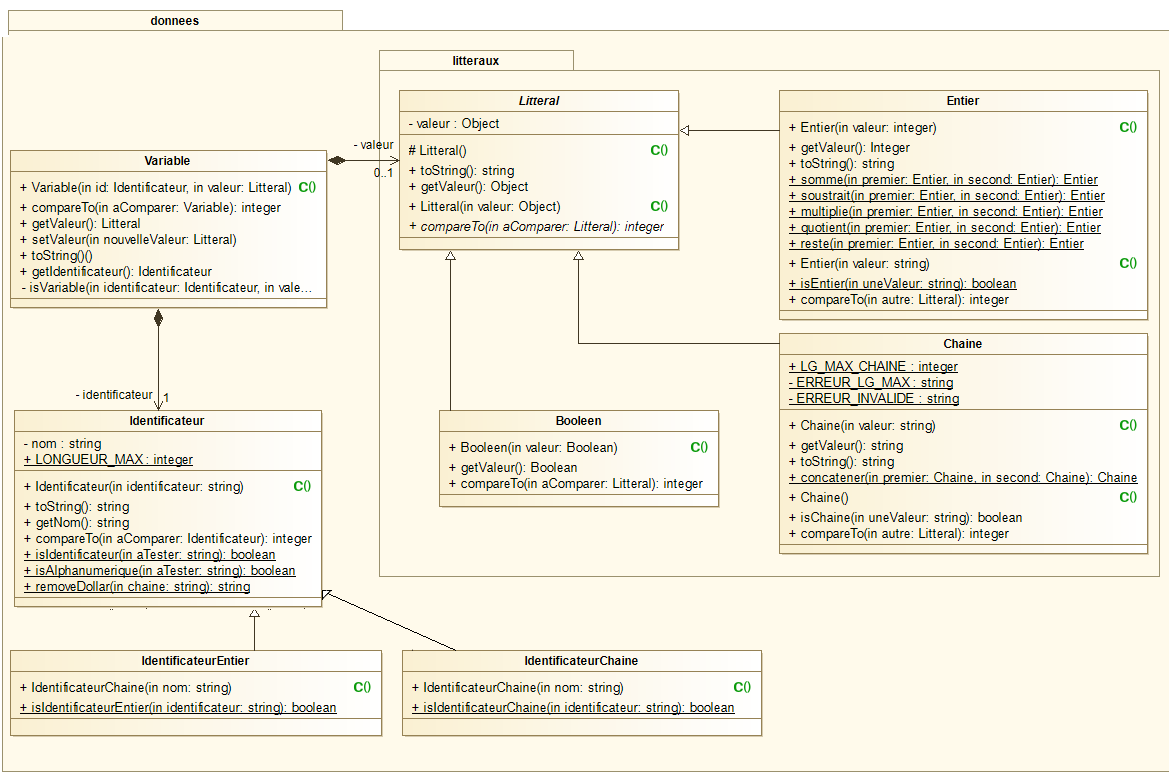
\includegraphics[scale=0.55]{./img/COO/PackageDonnees}

\section{Paquetage interpreteurlir.expressions}
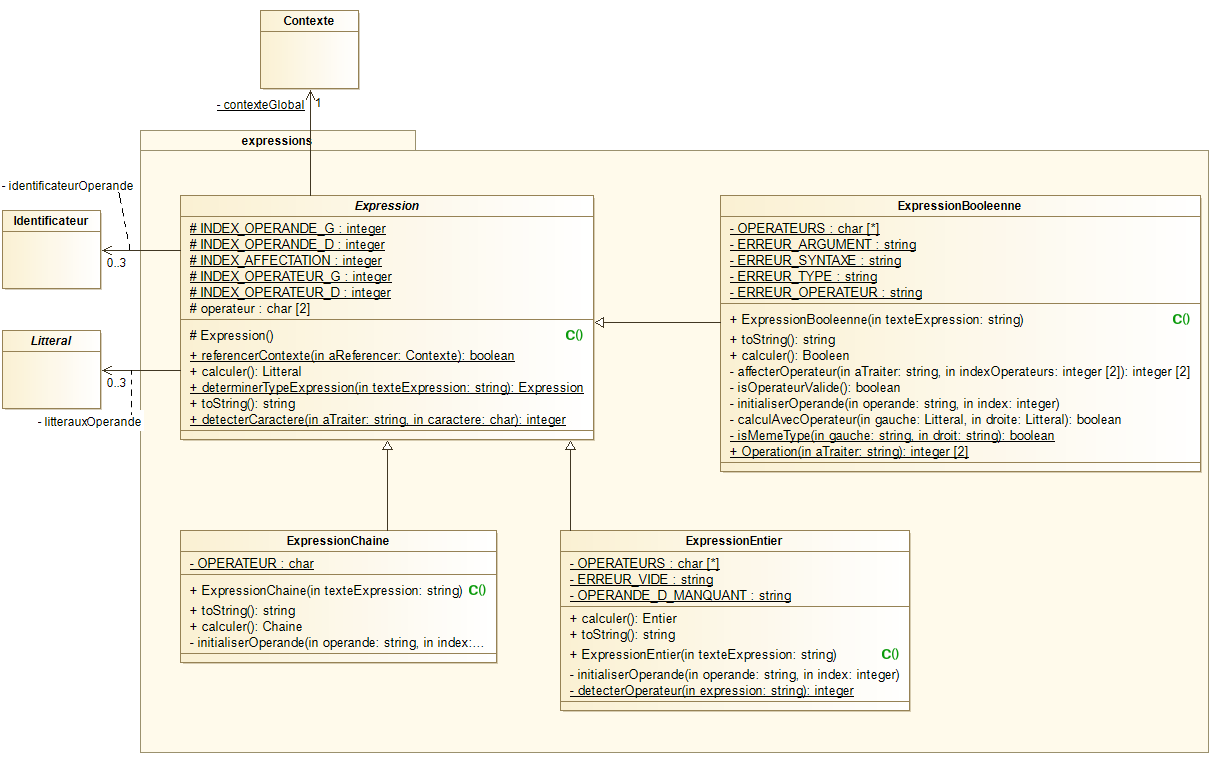
\includegraphics[scale=0.55]{./img/COO/PackageExpression}

\section{Paquetage interpreteurlir.programmes}
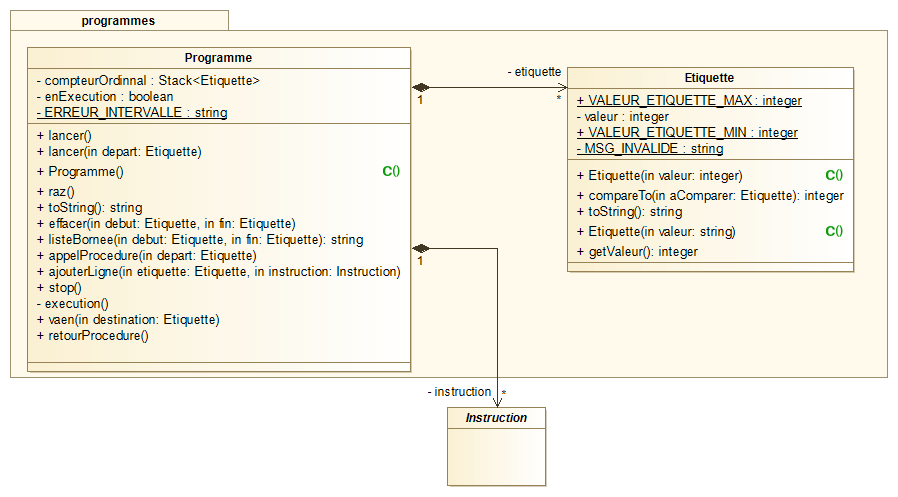
\includegraphics[scale=0.55]{./img/COO/PackageProgrammes}

\section{Paquetage interpreteurlir.motscles}
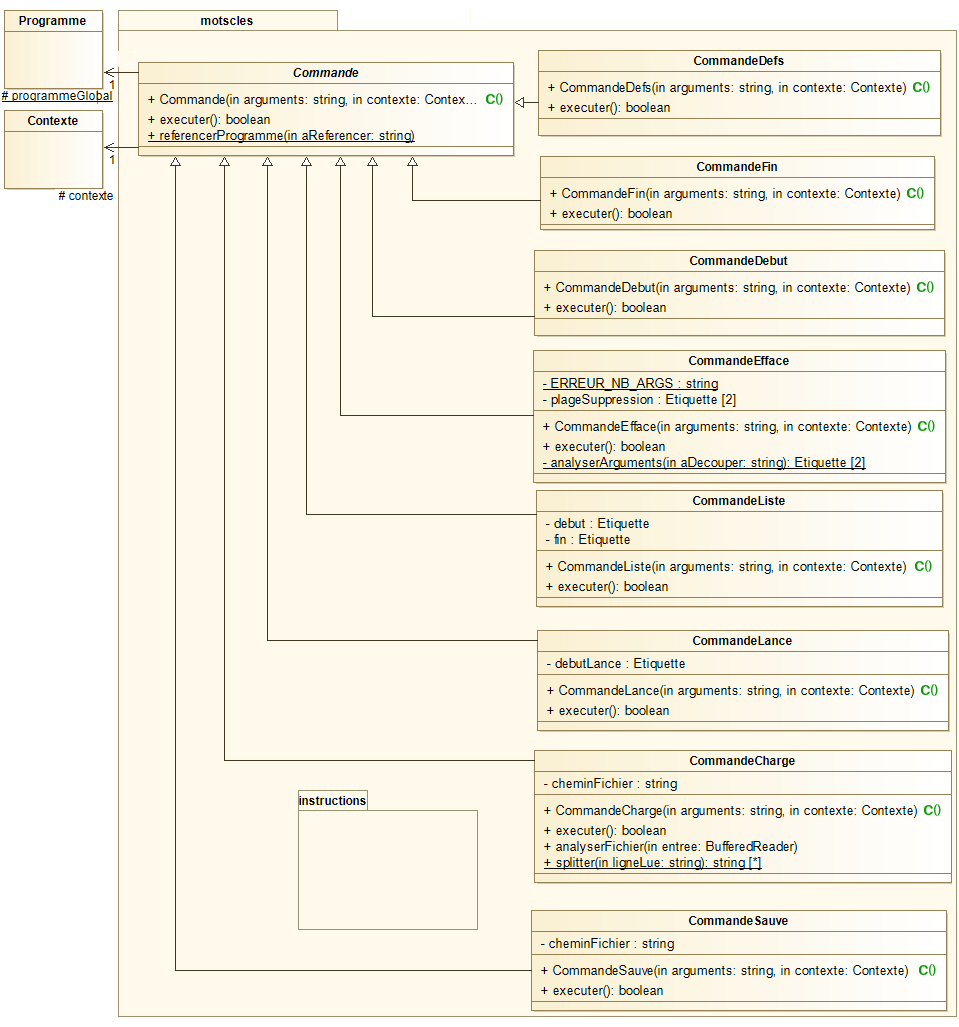
\includegraphics[scale=0.60]{./img/COO/PackageMotscles}

\section{Paquetage interpreteurlir.motscles.instructions}
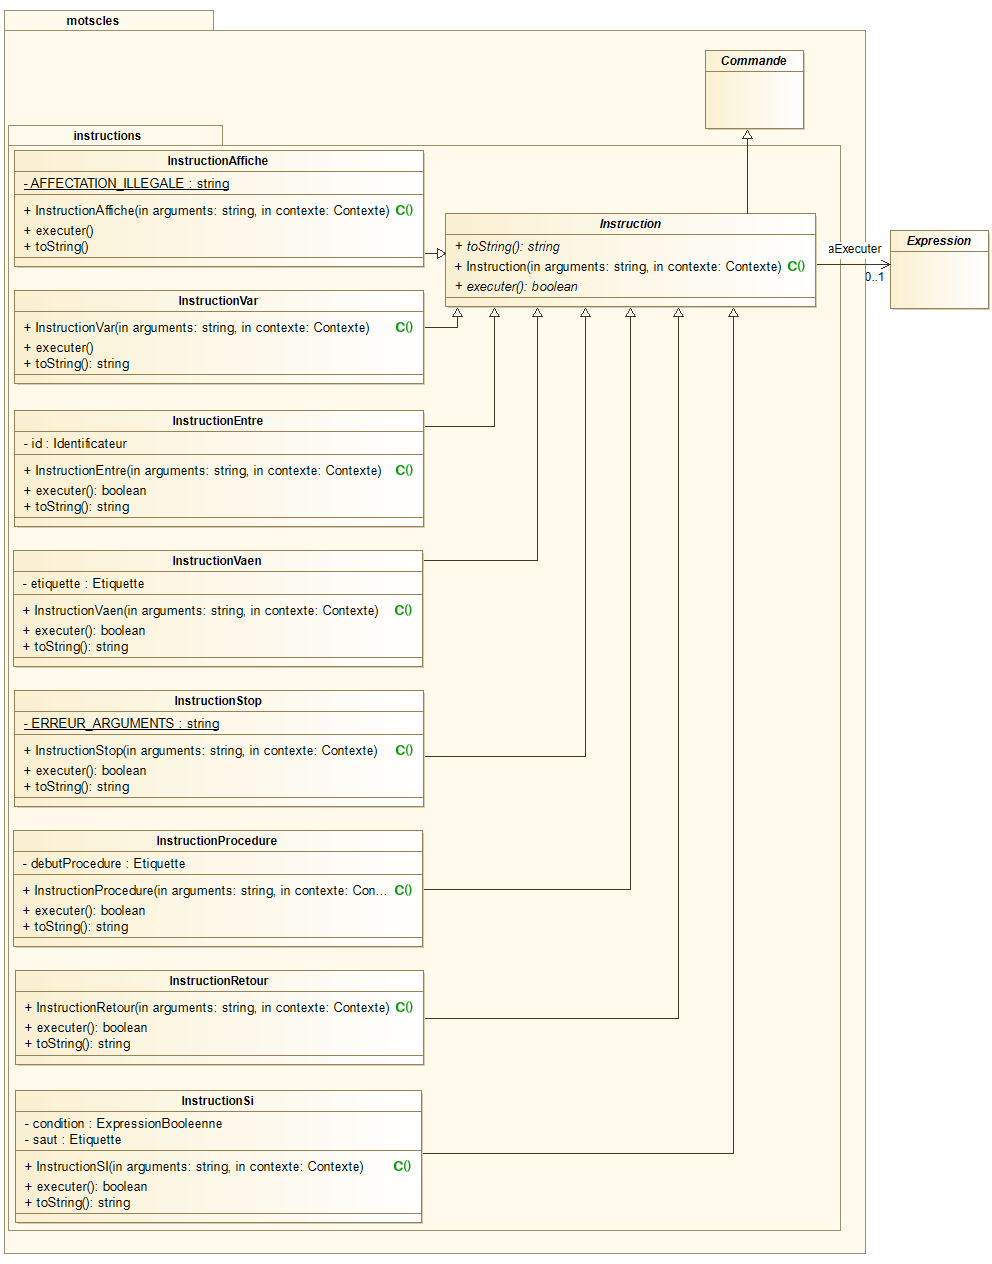
\includegraphics[scale=0.60]{./img/COO/PackageInstruction}

\section{Paquetage interpreteurlir}
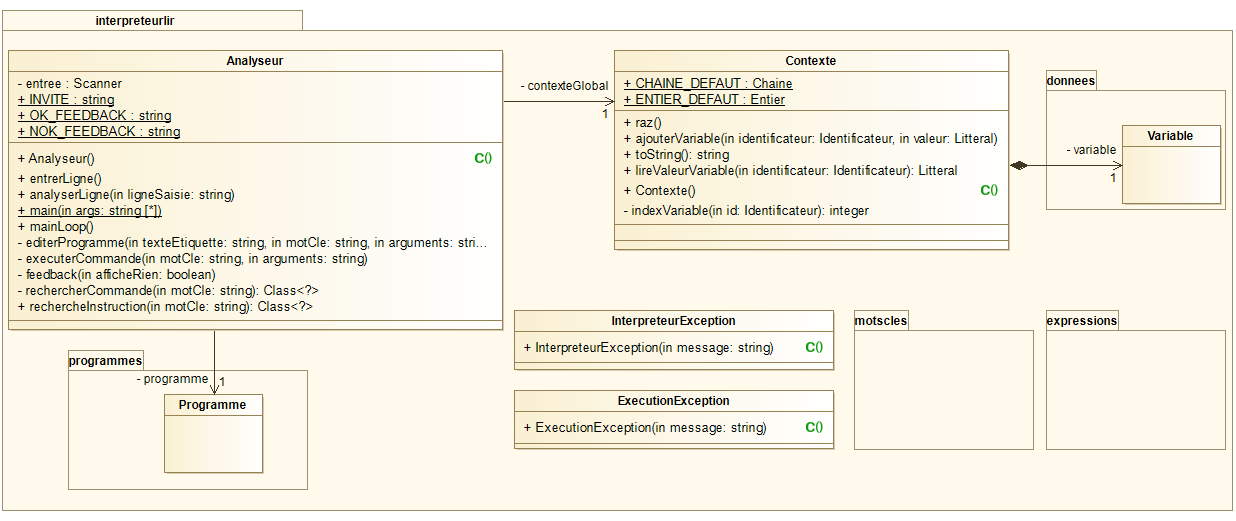
\includegraphics[scale=0.55]{./img/COO/PackageInterpreteurlir}